\documentclass[12pt]{article}
\usepackage{natbib} % Tidies up citation numbers.
\usepackage{url} % Provides better formatting of URLs.
\usepackage[utf8]{inputenc} % Allows Turkish characters.
\usepackage{graphicx}
\graphicspath{{./media}}
\usepackage[brazil]{babel}  
\usepackage[nopostdot]{glossaries}
\setglossarystyle{altlist}
\usepackage{hyperref} 

\usepackage{xcolor}%Allows highlighting text
\newcommand{\rascbegin}{\color{red}}    %rascbegin para iniciar a marcação de um rascunho
\newcommand{\rascend}{\color{black}}    %rascend para terminar de marcar um rascunho
%rascunhos em vermelho e definitivos em preto

%\hyphenation{op-tical net-works semi-conduc-tor} % Corrects some bad hyphenation 
\makenoidxglossaries

\loadglsentries{glossario}

%\makeglossary
\newcommand{\Aa}{\textit{Aedes aegypti}}

\begin{document}
	%\begin{titlepage}
	% can use linebreaks \\ within to get better formatting as desired
	
	\title{Modelo de relatório sobre projeto de desenvolvimento e avaliação de artefatos de sistemas de informação para a Sala de Situação em Saúde da Faculdade de Ciências da Saúde da UnB baseado na Ciência do Projeto (\textit{Design Science}), V. 4.6}
	
	
	% author names and affiliations
	
	\author{Gabriel Alves Castro - 17/0033813 \and Pedro Lucas Pinto Andrade - 16/0038316 \and Tiago Cabral de Faria - 16/0146712}
	
	\date{8 de novembro de 2019}
	
	% make the title area
	\maketitle
	\tableofcontents
	\listoffigures
	\listoftables
	\printnoidxglossary
	
	
	%\end{titlepage}
	
%	\IEEEpeerreviewmaketitle
	
	\begin{abstract}
		\rascbegin
		Este documento apresenta um modelo para entrega do relatório final da disciplina Sistemas de Informação, turma A, semestre 2019.2, do Departamento de Ciência da Computação do Instituto de Ciências Exatas da Universidade de Brasília, executada sob responsabilidade do Professor Jorge Henrique Cabral Fernandes. 
		O relatório final da disciplina é o registro, na forma de relatório, da realização de um projeto de desenvolvimento e avaliação de artefatos de sistemas de informação para a Sala de Situação em Saúde da Faculdade de Ciências da Saúde da UnB. 
		Os artefatos visam solucionar alguns dos problemas com informação relacionados ao funcionamento da Sala de Situação da FS/UnB.
		O projeto adere à abordagem de ciência do projeto (\textit{Design Science}). 
		Este modelo descreve as seções que devem fazer parte do relatório.
		Orientações adicionais para desenvolvimento do relatório e de seu correspondente projeto, com critérios de execução do projeto, avaliação do relatório, atribuição de pontos etc, encontram-se no docu\-mento de ``Orientação''.
		\rascend
	\end{abstract}	
	
	
	\section{Identificação do problema de design\label{Sec:CP:IdentifProblema}}
	
	O projeto a ser desenvolvido pelos integrantes da equipe consiste em aprimorar um artefato já existente identificado na Sala de Situação do CENTEIAS (Faculdade de Saúde da Universidade de Brasília - FS). Os participantes da Sala de Situação têm interesse em acessar informações sobre as epidemias e palavras chave de interesse, a partir de publicações da rede social Twitter, pelo público geral. No entanto o grande volume de publicações, devido ao alto uso da mídia social Twitter, impossibilita o acesso e processamento tempestivo desses dados, com forma manual de busca.
	
	Para identificação do problema \textit{design}, é adotada a abordagem de [Wieringa, 2014, 15-17]. Assim sendo, descremos abaixo as prioridades dos fluxos de trabalho: 
	\begin{enumerate}
    \item Melhoria do projeto já implementado com o refatoramento do código já existente de busca de twetts;
		\item Por meio da implementação de um modelo de mineração de textos com parâmetros estabelecidos que melhorem a acurácia do twittes considerados úteis;
		\item De tal forma que a filtragem de dados seja realmente relevante;
		\item E com isso o cliente tenha uma ferramenta de fácil utilização (com o desenvolvimento de um Front-End amigável) facilitando assim o uso do artefato por qualquer membro do CENTEIAS.
        \end{enumerate}
	
	As subseções seguintes definem o que deve estar presente no detalhamento da declaração do problema de \textit{design}.
	
	\subsection{Contexto de problemas com informação\label{contexto}}
    O CENTEIAS, Centro de Tecnologias Interativas em Saúde, tem como objetivo prover a Faculdade de Saúde (FS) da UnB um espaço transdisciplinar de suporte para ensino, pesquisa e extensão, buscando estabelecer parcerias com diversos institutos e faculdades da UnB e de outros locais do Brasil e do mundo. (citar site FS)
    
    A Sala de Situação em Saúde da FS, hospedada dentro do laboratório do CENTEIAS, realiza coleta e análise de dados epidemiológicos do Brasil e do mundo. A análise desses dados é feita com a missão de identificar crises e surtos relacionados à saúde pública que podem estar ocorrendo, ou que podem vir a ocorrer futuramente. Dessa forma, é possível organizar políticas de prvenção e contenção destes surtos para minimizar os danos causados pelos mesmos.
    
    A Sala de Situação hoje desenvolve vários produtos, como:
    \begin{enumerate}
        \item Boletins Epidemiológicos
        \item Boletins de Monitoramento
        \item Boletins Consolidados
        \item \textit{Clippings} de Notícias
    \end{enumerate}
    A equipe da Sala de Situação expressou interesse em coletar dados de fontes mais imediatas e diretas como a rede social Twitter, onde a população publica informações em tempo real sobre acontecimentos gerais.
    
    Atualmente, a Sala de Situação possui uma ferramenta de busca de informações por palavras-chave na rede social Twitter, desenvolvido por Alvarez e Vale \rascbegin(citar Alvarez e Vale) \rascend durante o primeiro semestre de 2019. O sistema busca e armazena tweets com determinadas palavras-chave designadas pelo usuário. Entretanto, devido a dificuldades de implementação e infraestrutura, a forma de uso do sistema ficou pouco prática. Além dessa complexidade para o uso, os dados coletados são exportados em um formato de difícil visualização, necessitando de um alto custo de tempo para analisar esses dados.
    
    
    


	\subsection{Tratamento desse contexto com um artefato dese\-nhado ou redesenhado\label{tratamento}}
	
	Para suprir o interesse expressado da equipe da sala de situação em coletar dados úteis do Twitter, planejamos melhorar o artefato desenvolvido por Alvarez e Vale através de um redesenho de seu funcionamento. Pretendemos:
	\begin{itemize}
	    \item Utilizar o sistema de buscas existente, complementando-o com filtros mais eficientes
	    \item Adicionar alguma capacidade de mineração de texto para extrair informações relevantes dos dados
	    \item Fornecer uma forma de visualização clara das informações coletadas
	\end{itemize}
	
	O artefato redesenhado será executado pela equipe da sala de situação, que fornecerá as palavras desejadas para a busca e depois poderá analisar os resultados por meio de uma interface web.
	
	
	
	\subsection{Artefato atende a um conjunto de características (requisitos de alto nível)\label{requisitos:alto:nivel}}
	
	A principal característica a ser atingida pelo sistema é o seu funcionamento robusto, para proporcionar à sala de situação uma forma de acesso à fonte de informações desejada. Para complementar esse requisito, uma interface clara tanto para a configuração e execução do buscador, assim como para a análise dos dados recolhidos é de grande necessidade, para dar usabilidade ao artefato. Além disso, os dados devem ser minimamente processados e filtrados para que mantenham sua relevância à equipe do CENTEIAS.
	

	\subsection{Contribui para o alcance de determinadas metas para as partes interessadas (\textit{stakeholders})\label{metas:stakeholders}}
	
	Com o artefato atendendo os requisitos funcionais descritos, a equipe da sala de situação do CENTEIAS terá acesso eficiente e prático a uma grande fonte de informação rápida, a rede social Twitter, aumentando a sua capacidade de analisar e tomar decisões sobre problemas de saúde pública que possam estar ocorrendo em qualquer local. A equipe terá uma ferramenta a mais em seu arsenal para prever epidemias ou outros casos em saúde que necessitam de ações rápidas.
	
	
    
	\section{Conscientização do problema\label{Sec:CP:ConscientizProblema}}
	
	
	
	\subsection{Problema atual}
	
	Redes sociais estão repletas de usuários se comunicando a todo momento, gerando uma grande quantidade de dados. Se conseguirmos processar esses dados, podemos extrair informações úteis sobre diversos assuntos e utilizar essas informações para, por exemplo, observar sinais de crises de saúde que possam estar prestes a ocorrer. Esse é o objetivo da equipe da sala de situação do CENTEIAS.
	
	Com esse objetivo de recorrer às redes sociais como uma fonte de informação adicional, surge o problema enfrentado pela equipe. A sala de situação precisa receber informações relevantes da busca na rede social, sendo o Twitter a rede escolhida, para posteriormente analisar o que foi recebido e tomar decisões sobre o que for observado. O artefato atual que está implementado na sala de situação, desenvolvido por Alvarez e Vale no período 2019.1 \rascbegin(citar Alvarez e Vale) \rascend não está solucionando o problema de forma satisfatória para o cliente, por isso estamos propondo o redesenho do mesmo para solucionar a necessidade da equipe.
	
	
	
	\subsection{Proposta de eliminação de um problema}
    
    \begin{figure}[ht]
    \centering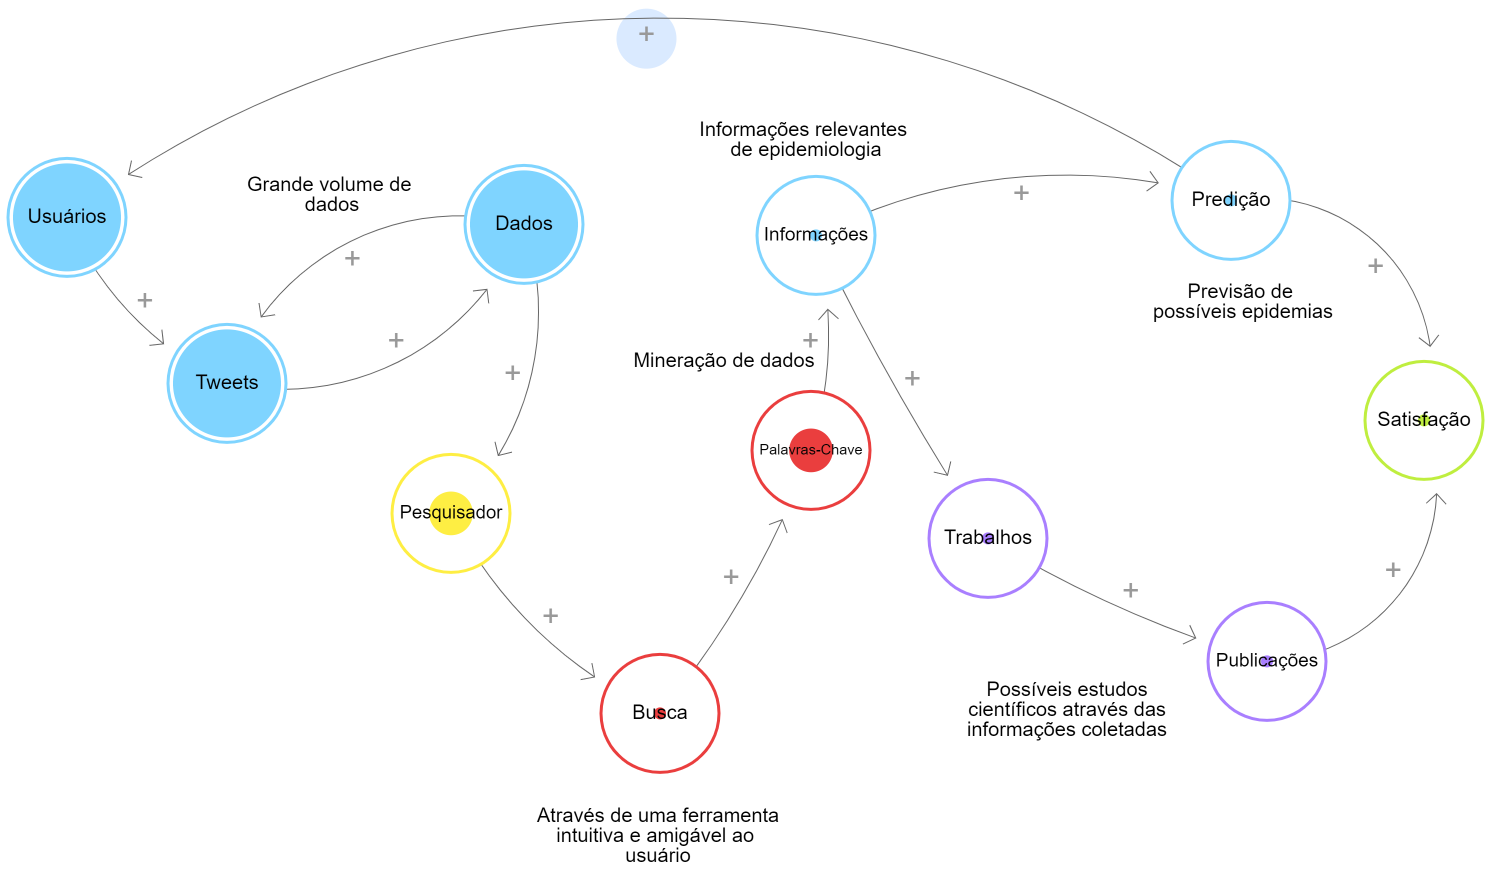
\includegraphics[width=1\textwidth]{media/diagrama_causal.png}
    \caption{Efeito da captura automática de tweets na sala de situação. Ver simulação em \url{https://bit.ly/30VeTas}\label{causal1:solucao}}
    \end{figure}
    
    
    A figura 1 apresenta o impacto do artefato proposto, ou seja, do software redesenhado tendo como base o de Alvarez e Vale, na sala de situação. Podemos por meio dela observar como o artefato será útil para solucionar o problema do cliente e garantir a satisfação do mesmo, por meio do cumprimento dos requisitos funcionais descritos. O software que pretendemos entregar influenciará as duas esferar vermelhas no diagrama, a interface intuitiva e a mineração de dados, que por meio das relações descritas no mapa, irão garantir a satisfação do cliente.
    
    
    
	\subsection{Declaração precisa dos limites do aprimoramento}
	
	O artefato que estamos propondo, como dito anteriormente, tem como objetivo proporcionar à equipe da sala de situação o acesso a dados da rede social Twitter para retirar informações úteis para a análise da saúde pública no Brasil e em outros locais. Portanto, o software não será capaz de realizar todo o trabalho da equipe, ficando por encargo dessa tarefas como: 
	\begin{itemize}
	    \item Escolher palavras chave que sejam de interesse;
	    \item Analisar as informações obtidas;
	    \item Extrair, das informações obtidas, o conhecimento que lhe for útil;
	    \item Usar esse conhecimento para o fim desejado;
	\end{itemize}
	Assim, como um martelo, o artefato proposto não será capaz de realizar todo o trabalho sozinho, mas será uma ferramenta que deve ser utilizada pela euqipe do CENTEIAS para auxiliar o trabalho de extrair informações desejadas do Twitter.
	
	
	
	\section{Identificação dos artefatos\label{Sec:CP:IdentifArtefatos}}
	\subsection{Busca de Tweets de Alvarez e Vale}
	Para realizar a busca de tweets, iremos utilizar o artefato desenvolvido por Alvarez e Vale \rascbegin(citar Alvarez e Vale) \rascend que já está presente na sala de situação. Este é o artefato sobre o qual estamos projetando nosso redesenho, com o objetivo de ampliar a sua proposta de busca de tweets por meio do processamento dos dados que já são obtidos pelo mesmo e da inclusão de uma interface amigável para o usuário. Esse é  artefato que será de maior utilizade para nossa proposta.
	
	Para realizar a busca e captação de tweets, o artefato citado utiliza uma biblioteca da lingugagem Python chamada Tweepy, que facilita todo o processo de conectar ao Twitter e receber informações do mesmo.
	
	
	\subsection{Tweepy}
	Tweepy é uma biblioteca desenvolvida para a linguagem Python que tem como objetivo facilitar o acesso a API do Twitter. Ela nos dá a capacidade de conectar ao Twitter, fazer buscas e baixar tweets, exatamente o que precisamos para coletar informações da rede social. O Twitter possui limitações ao período que pode ser acessado, sendo possível captar apenas tweets que estão sendo postados no momento em que a ferramenta está sendo executada, todavia isso não será um problema para nosso artefato, já que o grande objetivo de coletar dados do Twitter é o acesso em tempo real à informação.
	
	\subsection{Django}
	Django é um framework web para Python que foi criado com o objetivo de proporcionar o desenvolvimento rápido de aplicações web. Será útil para a criação de uma interface amigável e rápida para o artefato, que facilitará o uso da ferramenta pela equipe do CENTEIAS.
	
	\rascbegin
	
	
	\paragraph{Uso da UML - Unified Modeling Language} As relações entre os usuários da Sala de Situação e os artefatos já existentes na Sala devem ser apresentadas por meio de diagramas de caso de uso na UML, que indicam que tipo de uso é feito, ou deveria ser feito, para os artefatos identificados.
	Para uma breve introdução aos diagramas UML de casos de uso recomenda-se o trabalho de \citet{lucidchart_modelos_2019}. A figura \ref{caso:de:uso} apresenta um exemplo de diagrama de caso de uso em UML, que ilustra as relações entre usuários e um possível artefato (inexistente) denominado ``Sistema de Gerenciamento de Notícias e Clippings''.
	
	\begin{figure}[ht]
		\centering
		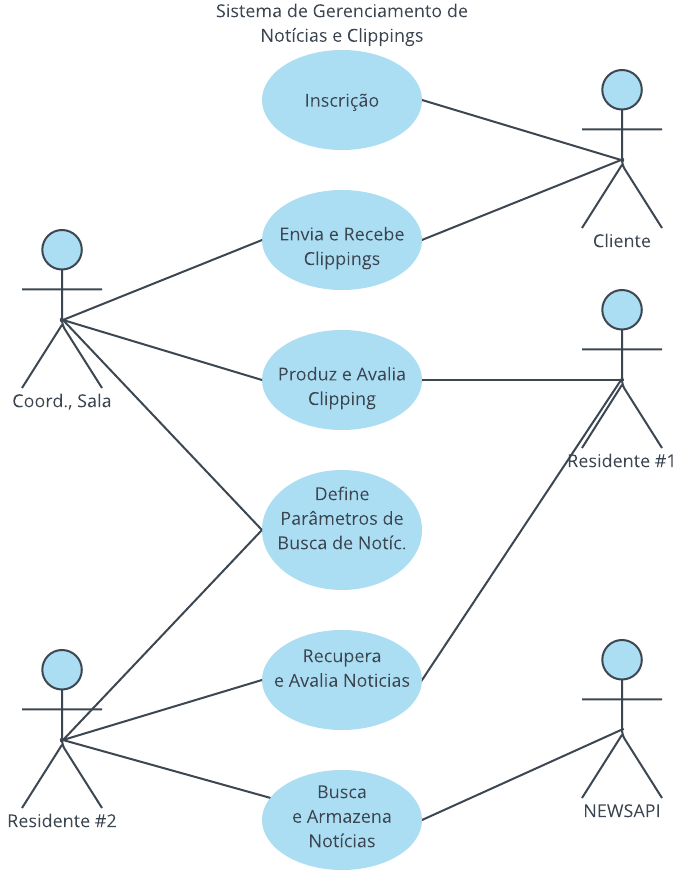
\includegraphics[width=0.5\textwidth]{CasodeUsoparaaSaladeSituacao.png}
		\caption{Diagrama de casos de uso para um possível artefato (inexistente) denominado ``Sistema de Gerenciamento de Notícias e Clippings''\label{caso:de:uso}.}		
	\end{figure}
	
	O desenho dos diagramas UML de casos de uso nesta seção ainda pode ser feito à mão, e posteriormente fotografado e inserido no relatório neste estágio de produção do mesmo, mas
	recomenda-se fortemente o registro gratuito e uso do aplicativo Lucid Chart, em sua versão gratuita, para produção dos diagramas que devem estar nesta seção do relatório, bem como nas seções seguintes.
	
	\rascend
	
	\section{Proposição de artefatos\label{Sec:CP:ProposicaoArtefatos}}
    O acesso a dados relevantes e em tempo útil é de grande importância para o trabalho da equipe da sala de situação do CENTEIAS, ncessidades que o artefato de Alvarez e Vale conseguiu suprir. Entretanto, a forma como foram atingidos esses objetivos não foram satisfatórias para o cliente, que não conseguiu tirar proveito das funcionalidades oferecidas pelo software.
    
    Nosso artefato almeja, portanto, expandir as funcionalidades já oferecidas pelo software de busca de tweets já presente na sala de situação. Para facilitar a integração com o artefato de Alvarez e Vale, utilizaremos a linguagem de programação Python para desenvolver um projeto aprimorado, que será composto de:
    \begin{itemize}
        \item Busca de tweets por palavras chaves configuráveis;
        \item Análise dos tweets obtidos;
        \item Interface para análise dos dados por parte da equipe;
    \end{itemize}
    
    O artefato será executado em uma máquina conectada à rede da sala de situação do CENTEIAS, que atuará como um servidor, sendo o mesmo um servidor dedicado ou não, e será acessado por meio da interface web de máquinas conectadas na mesma rede. A busca será executada e armazenada pelo servidor onde o software estiver sendo hospedado, sendo os parâmetros escolhidos por usuários nas máquinas conectadas por meio da interface. O desempenho do software dependerá em grande parte de quanto tempo o mesmo se manter em execução coletando dados para serem processados.
    
    \subsection{Elaboração da Composição do Artefato}
    \subsubsection{Busca de Tweets}
    A busca de tweets será realizada como já está sendo feita pelo software em que estamos baseando nosso redesenho. O artefato realiza a busca de forma automatizada por palavras chaves determinadas pelo usuário, sendo mais rápida e prática que uma busca manual \rascbegin(citar Alvarez e Vale)\rascend. A busca então continuará utilizando a biblioteca Tweepy, como foi desenvolvida, com alguns pequenos ajustes para facilitar a análise posterior dos tweets, caso se mostrem necessários.
    
    \subsubsection{Análise dos Tweets}
    Para analisar os tweets utilizaremos técnicas de mineração de texto para gerar uma análise de sentimentos georeferenciada. Uma análise de sentimentos é a extração de sentimentos e emoções de um texto em linguagem natural \rascbegin(citar fonte sobre Análise de sentimentos)\rascend. Essa análise pode ser de grande importância ao analisar uma fonte de informações tão informal como o Twitter, principalmente considerando a finalidade com que os tweets serão analisados. Ter conhecimento sobre a emoção com que um determinado grupo de pessoas falou sobre um dos assuntos sendo buscados fornece mais poder à equipe da sala de situação para entender o que pode estar ocorrendo em determinado local, em relação a este assunto.
    
    \subsubsection{Interface}
    Uma interface clara e amigável é de grande importância para manter a utilidade da ferramenta para a equipe do CENTEIAS. Além de facilitar a configuração das palavras chaves que serão utilizadas na busca e a execução da mesma, a interface também fornecerá uma forma fácil de visualizar os dados gerados. Os tweets capturados serão agrupados por seu local de origem, sendo assim possível ter uma visão georeferenciada do volume de pessoas falando sobre o assunto determinado pelo usuário da ferramenta. Além disso, será também mostrado a análise dos sentimentos que foi gerada durante a etapa de análise, também de forma georeferenciada, para auxiliar no entendimento da sensação da população sobre o assunto. Para atender a essas característica, a interface será uma interface web desenvolvida no framework Django.
    
    \subsection{Viabilidade do Artefato}
    Como a etapa de busca de tweets será reutilizada, com pequenas modificações onde necessário, do artefato desenvolvido por Alvarez e Vale, não há grande necessidade de código a ser escrito para atender a essa parte do artefato.
    
    A interface será desenvolvida no framework web Django, que tem como objetivo o desenvolvimento rápido de páginas web sem grande necessidade de código. O esforço nessa etapa se mostra então no aprendizado da ferramenta para ser utilizada, e não no desenvolvimento da interface em si.
    
    A análise de tweets se mostra a mais complexa, pois irá necessitar de mineração de texto para processar e gerar a análise de sentimentos. Essa será a etapa que necessitará de mais esforço para ser desenvolvida de forma a atender a proposta do artefato.
    
    Com isso, apesar de necessitar elaboração de código não trivial e de tempo para ser desenvolvido, o artefato aparenta ter sua implementação viável dentro do tempo esperado pelo cliente.
    
    
    
    
    \rascbegin
    INCLUIR DIAGRAMAS DE CASOS DE USO SEGUINDO A UML
    \rascend

	\section{Projeto dos artefatos selecionados\label{Sec:CP:ProjetoArtefato}}
    \rascbegin	
	Nesta seção o relatório registra o projeto técnico dos artefatos selecionados para desenvolvimento no item \ref{Sec:CP:ProposicaoArtefatos}, 
	por meio do qual será evidenciada a adoção de métodos, técnicas e ferramentas para desenvolvimento de artefatos de software, tais como:
	\begin{itemize}
		\item Métodos e técnicas para conteinerização de aplicações e criação de soluções de Plataformas como Serviço (\textit{Platform as a Service - PaaS}) com Docker \citep{matthias_docker:_2015,mouat_using_2016};
		
		\item Métodos e técnicas para desenvolvimento de bases de dados como PostgreSQL, MySQL etc;
		
		\item Métodos e técnicas para desenvolvimento de APIs com Swagger \citep{swagger_swagger_2018} e aplicações web RESTFull\citep{mehta_restful_2014};
		
		\item Métodos e técnicas para desenvolvimento de arquiteturas web \citep{adams_mastering_2015,firtman_high_2015};
		
		\item Métodos e técnicas para desenvolvimento ágil de software \citep{garbajosa_agile_2018,lacey_scrum_2012}, seus requisitos \citep{davis_software_1990} e testes \citep{rose_cucumber_2015,smart_bdd_2014};
		
		\item Métodos e técnicas para utilização de ambientes avançados de desenvolvimento de software com Jira \citep{li_jira_2015}, Confluence \citep{kohler_atlassian_2013} e Bitbucket/GIT  \citep{westby_git_2015};
		
		\item ou quaisquer outros métodos e técnicas aos quais tenha tido acesso ou possa desenvolver durante o projeto.
	\end{itemize} 
	
	Deverão ser apresentados e descritos diagramas arquiteturais em UML que detalhem o projeto técnico dos elementos, usando diagramas UML de implantação, componentes, atividades, estados, comunicação, objetos, classe, sequência e (ou) casos de uso.
	
	Para uma breve introdução aos diagramas da UML recomenda-se a consulta a uma ou mais das três fontes de informação seguintes:
	\begin{itemize}
		\item Página de ``Modelos e exemplos de diagramas UML'' da \citet{lucidchart_modelos_2019}, que oferece um breve guia da UML 2.0 e uma ferramenta online extremamente conveniente para a edição de diagramas UML \citep{lucidchart_work_2018}. Recomenda-se fortemente o registro gratuito e uso do aplicativo Lucid Chart , em sua versão gratuita, para produção dos diagramas que devem estar nesta seção do relatório;
		\item ``Resumo dos Diagramas UML'', de \citet{figueiredo_resumo_2019}, que apresenta em poucos slides breves definições e exemplos da utilidade de cada um dos principais diagramas da UML; e
		\item ``UML 2.0: Guia Prático'' de \citet{guedes_uml_2014}, que apresenta em onze páginas um breve exemplo da utilidade de cada um dos principais diagramas da UML.
	\end{itemize}
	
	\section{Desenvolvimento do artefato\label{Sec:CP:DesenvArtefato}}
	
	Esta seção do relatório registra de que forma se deu a codificação dos artefatos selecionados para desenvolvimento no item \ref{Sec:CP:ProjetoArtefato}, usando linguagens de programação e ferramentas diversas.
	
	Será responsabilidade da equipe criar um ambiente de desenvolvimento de software simples, mas efetivo, para produzir um ou mais artefatos que possam ser colocados em uso no ambiente computacional da Sala de Situação.

	Os artefatos desenvolvidos devem ser 
	registrados em um repositório de código de livre acesso, na plataforma github. Todos os membros da equipe devem fazer contribuições ao repositório de código.
	
	Os artefatos desenvolvidos devem ser empacotados por meio de uma imagem de contêiner, utilizando a tecnologia Docker \citep{linuxtips_docker_2015,matthias_docker:_2015} e para uso do sistema operacional Linux.
	
	No registro do desenvolvimento devem ser apresentadas as análises de \textit{commits} realizados no repositório Git, usando as ferramentas automatizadas de análise do próprio Git, onde deve ser destacada a contribuição de cada um dos membros do grupo para a construção dos artefatos, inclusive a documentação dos mesmos.
	
	Devem ser estimados os esforços de cada membro em termos de horas de trabalho para o desenvolvimento.
	
	\section{Implementação do artefato\label{ImplArtefato}}
	
	Esta seção registra como se deu a colocação do artefato em pleno funcionamento operacional no ambiente organizacional da Sala de Situação da FS/UnB.
	
	A imagem ``conteinerizada'' do artefato será instalada em um ambiente operacional de TI, por equipe da própria Sala de Situação ou pela própria equipe de projeto, conforme os acordos estabelecidos entre as partes.
	
	Uma vez que estejam instalados no ambiente computacional, os artefatos em funcionamento devem ser apresentados, com instruções para a utilização do artefato pela própria equipe da Sala de Situação, em data e horário previamente agendado.
	
	Dúvidas devem ser esclarecidas, e a equipe da Sala de Situação terá sete dias para utilizar o artefato, após o que será feita a avaliação.
	
	O registro desse processo de implementação deve ser detalhadamente apresentado.
	
	\section{Avaliação do artefato\label{Sec:CP:AvalArtefato}}
	
	Esta seção registra a avaliação do impacto do(s) artefato(s) desenvolvido(s) e implementado(s) no ambiente operacional da Sala de Situação.

	Para tal, em aderência à proposta de \citep{dresch_design_2015}, será feita a observação e avaliação do artefato enquanto solução satisfatória para o problema.
	Serão revisados, pela equipe do projeto em conjunto com a equipe da Sala de Situação, todos os requisitos de solução que foram declarados em passos anteriores, a fim de avaliar se eles foram atendidos.

	A avaliação será realizada junto aos usuários potenciais ou reais dos artefatos desenvolvidos. 

	Serão observadas e registradas as condições técnico-computacionais de execução efetiva do artefato junto ao cliente.

	Será acompanhada a demonstração de funcionamento do artefato, o auxílio à operação do artefato pelos usuários, e conduzida a discussão consensual sobre atendimento aos requisitos do problema.

	Será observada a operação efetiva do artefato por usuários, em situação real ou simulada.

	Será feita discussão e consenso com a equipe de usuários/avaliadores, sobre o grau de atendimento a cada um dos requisitos de solução do problema.

	Será feita declaração dos limites de satisfação do artefato, em relação ao planejado.

	Será feita declaração das limitações/potencialidades reais de funcionamento do artefato.
	Em caso de não atendimento aos requisitos da solução, será identificado em que passos anteriores foram introduzidas as falhas.
	
	\section{Explicitação das aprendizagens\label{Sec:CP:ExplicitAprendizagens}}
	
	Esta seção registra a explicitação das aprendizagens realizadas por todas as partes envolvidas no projeto.
	
	A equipe fará a declaração explicita dos fatores que contribuiram positivamente para o sucesso do projeto, bem como os fatores que falharam. Deve-se buscar relacionar esses fatores com os fatores e propostas de neutralização indicadas por \cite{prakken_information_2000}, conforme conceitualmente apresentados nos itens \ref{literatura:prakken:problemas} e \ref{literatura:prakken:neutralizadores}.
	
	Isso será feito em vinculação aos problemas registrados e aos artefatos desenvolvidos durante o projeto.
	
	\section{Conclusões\label{Sec:CP:Conclusoes}}
	
	Nesta seção devem ser registradas as conclusões da equipe sobre a realização do projeto.
	
	Serão indicadas as limitações da pequisa/projeto realizado, bem como a necessidade de partes do estudo que precisariam ser mais aprofundadas.
	
	A conclusão de um relatório técnico deve sintetizar o conhecimento que foi gerado a partir do projeto desenvolvido, ou seja, deve ser decorrência lógica natural do que está registrado nas seções anteriores do relatório. Deve conter um sumário dos elementos mais importantes pode ser tabulado.
	
	Acerca das recomendações na conclusão, essas deve ser ligadas a problemas e questões que ficaram pendentes de solução.
	
	\section{Generalização para uma classe de problemas\label{Sec:CP:Generalizacoes}}
	
	Nesta seção deve ser registrada a generalização dos conhecimentos produzidos pela equipe durante a realização do projeto.
	
	Será apresentado um argumento conclusivo e embasado por evidências obtidas durante o projeto, acerca da extensão, limitações e contextos de aplicabilidade dos artefatos desenvolvidos pela equipe, de suas funções, de sua arquitetura, para solução de uma classe de problemas com informação, relacionada com os distintos tipos de sistemas de informação.

	\section{Comunicação dos Resultados\label{Sec:ComunicResultados}}
	
	A etapa de comunicação dos resultados não gera seções no relatório final, pois é cumprida com a realização de três tarefas:
	\begin{enumerate}
		\item Desenvolvimento de slides em aderência ao pacote \LaTeX\ beamer, para apresentação dos resultados da equipe em sala de aula. Note que um modelo de edição do conteúdo dos slides já se encontra no arquivo ``textoslides.tex'', que acompanha este modelo de relatório. Para gerar os slides compile o arquivo ``main2.tex'', que também acompanha este modelo. Note também que o conteúdo dos slides inserido no arquivo ``textoslides.tex'' também é automaticamente inserido ao final deste modelo de relatório;
		\item Apresentação oral do projeto desenvolvido pela equipe, em sala de aula, com o auxílio dos slides gerados conforme a tarefa anterior, e com a presença de todos os seus integrantes; e
		\item Desenvolvimento pleno deste relatório e sua entrega completa, baseado no modelo aqui descrito, na correspondente tarefa do ambiente Aprender.UnB, conforme orientações fornecidas.
	\end{enumerate}
	
	\section{Declaração sobre a contribuição individual de cada um dos autores do relatório e sobre a não existência de conflitos de interesse\label{Sec:DeclaracaoNaoConflito}}
	
	Ao final, cada um dos membros da equipe deve declarar a sua contribuição individual para o projeto.
	
	\subsection{Declarações do autor Jorge Henrique Cabral Fernandes}
	
	Jorge Henrique Cabral Fernandes declara que contribuiu diretamente para a elaboração dos seguintes aspectos do relatório:
	\begin{itemize}
		\item Concepção dos objetivos e forma do relatório;
		\item Glossário;
		\item Resumo;
		\item Introdução;
		\item Texto e diagrama usados na definição do problema;
		\item Condições e restrições gerais do projeto;
		\item Esqueleto de revisão teórico-conceitual;
		\item Modelo de um meta-sistema de informação;
		\item Proposta de organização do relatório;
		\item Rubrica de avaliação;
		\item Síntese de questões usadas para avaliação do projeto; e
		\item Conclusões e recomendações.	
	\end{itemize}
	
	Em suma, Jorge Henrique Cabral Fernandes declara toda a elaboração deste relatório foi de sua própria autoria, exceção feita à produção de itens do glossário, que foram desenvolvidos em equipe.
	
	O autor agradece a colaboração dos alunos dos semestres 2019.1, 2018.2, 2018.1, 2017.1 e 20172, na participação da realização e aprimoramento da disciplina, e na realização de projetos que contribuem para a melhoria da saúde pública. Agradece também aos membros do laboratório Centeias (Centro de Tecnologias Educacionais Interativas em Saúde) da Faculdade de Ciências da Saúde da Universidade de Brasília, pela parceria nas investigações sobre sistemas de informação em saúde, bem como agradece o apoio e colaboração de membros da Subsecretaria de Vigilância em Saúde do DF, da Fiocruz e do Ministério da Saúde, pela colaboração técnica.
	
	De outra forma, o autor declara que todas as omissões e erros eventualmente existentes são de sua inteira responsabilidade.
	
	Por fim, o autor deste relatório declara que não existem conflitos de interesse não declarados, envolvidos na produção do relatório.
	
	\bibliographystyle{plainnat}
	\bibliography{SisInfoSaude}
	
	\appendix
	\section{Identificação do problema}
\begin{frame}{Proposta}
	\begin{itemize}
		\item Definição / exemplo 1
		\item Definição / exemplo 2
		\item Definição / exemplo 3
	\end{itemize}
\end{frame}

\section{Conscientização do problema}
	\begin{frame}{Relações causais sob análise}
		\centering
		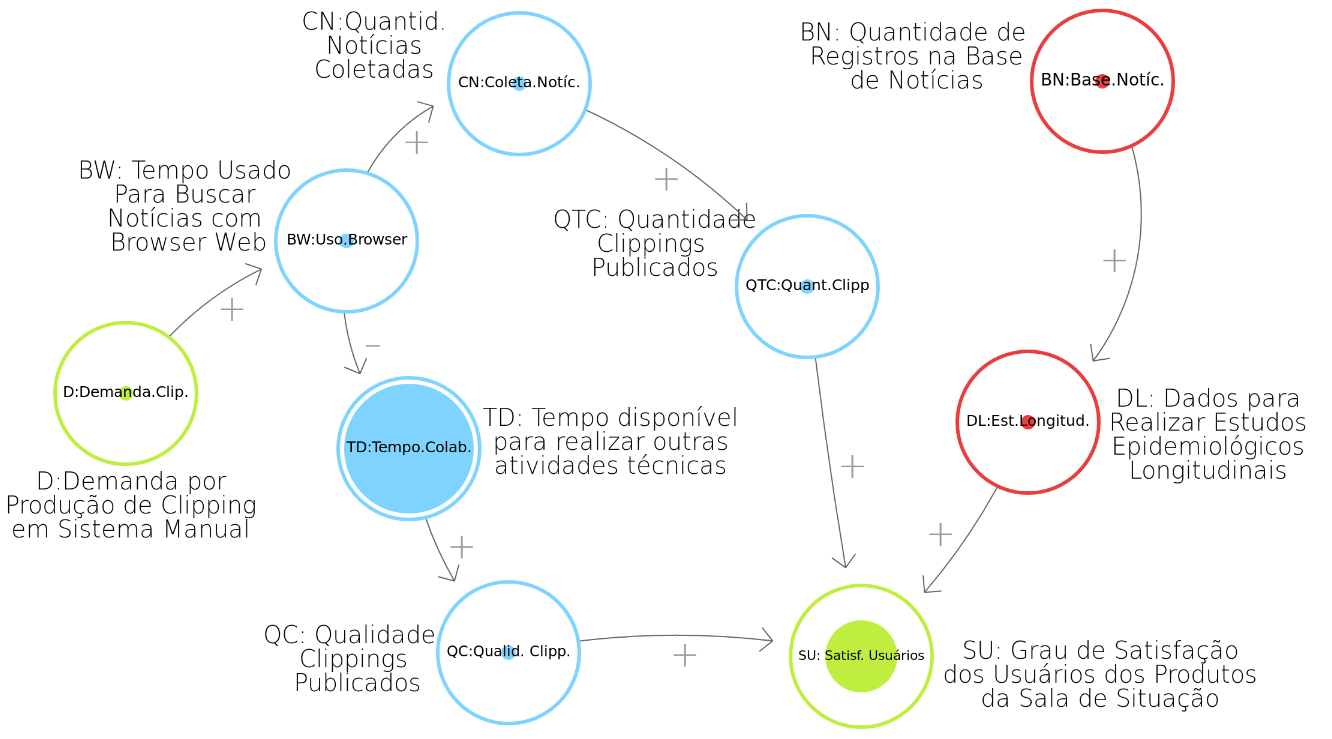
\includegraphics[width=0.8\textwidth]{ProducaoClippingManual.png}
	\end{frame}

%\section{Revisão da literatura}

\section{Identificação dos artefatos}
\begin{frame}{Artefatos Identificados}
	\begin{itemize}
		\item Definição / exemplo 1
		\item Definição / exemplo 2
		\item Definição / exemplo 3
	\end{itemize}
\end{frame}

\section{Proposição de artefatos}
\begin{frame}{Artefatos Propostos}
	\begin{itemize}
		\item Proposição / exemplo 1
		\item Proposição / exemplo 2
		\item Proposição / exemplo 3
	\end{itemize}
\end{frame}

\section{Projeto do artefato selecionado}
\begin{frame}{Projeto dos Artefatos}
	\begin{itemize}
		\item Diagrama / exemplo 1
		\item Diagrama / exemplo 2
		\item Diagrama / exemplo 3
	\end{itemize}
\end{frame}

\section{Desenvolvimento do artefato}
\begin{frame}{Atributos Técnicos dos Artefatos Desenvolvidos}
	\begin{itemize}
		\item Atributo / exemplo 1
		\item Atributo / exemplo 2
		\item Atributo / exemplo 3
	\end{itemize}
\end{frame}

\section{Implementação do artefato}
\begin{frame}{Como ocorreu a implementação?}
	\begin{itemize}
		\item Atributo / exemplo 1
		\item Atributo / exemplo 2
		\item Atributo / exemplo 3
	\end{itemize}
\end{frame}

\section{Avaliação do artefato}
\begin{frame}{Resultados das Avaliações}
	\begin{itemize}
		\item Resultado / exemplo 1
		\item Resultado / exemplo 2
		\item Resultado / exemplo 3
	\end{itemize}
\end{frame}

\section{Explicitação das aprendizagens}
\begin{frame}{O que o grupo aprendeu?}
	\begin{itemize}
		\item Aprendizagem / exemplo 1
		\item Aprendizagem / exemplo 2
		\item Aprendizagem / exemplo 3
	\end{itemize}
\end{frame}

\section{Conclusões}
\begin{frame}{Conclusões sobre a Realização do Projeto}
	\begin{itemize}
		\item Objetivos Alcançados? / exemplo 1
		\item Objetivos Alcançados? / exemplo 2
		\item Objetivos Alcançados? / exemplo 3
	\end{itemize}
\end{frame}

\section{Generalização para uma classe de problemas}
\begin{frame}{Generalização }
	\begin{itemize}
		\item Generalização / exemplo 1
		\item Generalização / exemplo 2
		\item Generalização / exemplo 3
	\end{itemize}
\end{frame}




	
	\section{Detalhamento dos projetos de artefatos\label{Sec:ProjetosArtefatosDetalhados}} \label{Mod:Processos:Graficos}
	
	Devem ser anexados ao final do relatório, nesta seção, todos os detalhamentos dos projetos de artefatos, tais como modelos de processos, modelos causais, protótipos de telas, modelos de dados de níveis conceituais, lógicos ou fisicos, diagramas UML, modelos de planilhas eletrônicas etc, tal como se apresenta o modelo de processo da figura ~\ref{FiguraGrande}.
	
	\begin{figure}[ht]
		\centering
		\includegraphics[page=208,width=1\textwidth,viewport=55 170 550 605,clip=true]{BPMN-2011-OMG-formal-11-01-03.pdf}
		\caption{Uma figura grande, que precisa ser colocada no final do relatório. fonte \citet[p. 178]{object_management_group_business_2011}\label{FiguraGrande}}
	\end{figure}
	\rascend
\end{document}
